\chapter[Reversible Universe]{Reversible Universe: Implications of Affordance-based Reverse Engineering of Complex Natural Systems}

%% FIXME - check proceedings references

\chapterauthor{Dominic Halsmer, Michael Gewecke, Rachelle Gewecke, Nate Roman, Tyler Todd, Jessica Fitzgerald}
\chapteraffiliation{Oral Roberts University}

\begin{abstract}
Recent advances in the field of engineering design suggest the
usefulness of the concept of affordance for reverse engineering of both
man-made and natural systems. An affordance is simply what a system
provides to an end-user or to another part of the system. With the
current recognition that engineering concepts are playing a key role in
deciphering the workings of complex natural systems such as the living
cell and the human brain, affordance-based reverse
engineering procedures should be considered as appropriate tools for this work. 
Such an approach may have important implications
for philosophy and theology.

Procedures for reverse engineering and design recovery have
become well-defined in several fields, especially computer software and
hardware, where pattern detection and identification play important
roles. These procedures can also be readily applied to complex natural
systems where patterns of multiple interacting affordances facilitate
the development, sustenance and education of advanced life forms such
as human beings. Thinking about the human condition in terms of
affordances leads to a new and fruitful interaction between the fields
of science and theology, in which the field of engineering plays a key
role in the dialogue. Proper understanding of the interplay between
both positive and negative affordances in the context of engineering
design under necessary constraints leads to a clearer worldview and a
better understanding of mankind{\textquotesingle}s place and purpose in
the universe.
\end{abstract}

\section{Introduction}

\index{reverse engineering|(}
\index{worldview}
\index{transcendentals}
\index{causation}
A worldview consists of what one believes to be true about the universe
and all of reality, including “how things work.”\footnote{Ken Samples gives a more technical description,
writing “A worldview forms a mental structure that organizes one’s
basic or ultimate beliefs. This framework supplies a comprehensive view
of what a person considers real, true, rational, good, valuable, and
beautiful” \citep{samples2007}.
Ron Nash defines worldview as “a conceptual scheme by
which we consciously or unconsciously place or fit everything we
believe and by which we interpret and judge reality” \citep[][p.~24]{nash1988}.
For a thorough treatment of the concept
of worldview, see David K. Naugle, \textit{Worldview: The History of a
Concept} \citep{naugle2002}.
} 
Worldviews are formed by mentally processing and filing away the
accumulated experiences of life. Inaccurate worldviews can prove
hazardous to one’s health. Although young children don’t know the
inverse square law of gravitation from physics, they learn very quickly
to respect the influence of gravity, or suffer the painful
consequences. Other aspects of reality take somewhat longer to
ascertain. But from the first moments of life, human beings enter this
world as little private investigators, gathering clues as to how the world
works. They are truth-seekers, especially when it comes to that which
brings satisfaction and enjoyment. Upon discovery of a new object, they
immediately embark on a crude type of reverse engineering exercise to
determine what can be known about this object and what uses it might
afford. Toddlers often go through a phase where they enjoy banging a
spoon against pots and pans. Perhaps this affords them an early
experience of understanding that they possess the power to control
their environment, to some small degree. Or maybe they just like to
make the banging sound. In either case, it results in increased
hand-eye coordination and knowledge of causation.

\index{reverse engineering!techniques!subtract and operate}
\index{stewardship}
\index{sustainability}
\index{curiosity}
\index{nature!comprehensibility}
As children get older and become more adept at reverse engineering
techniques, they often pass through a phase characterized by repeated
dissections of both natural and man-made objects. Perhaps taking apart
complex organisms/devices facilitates the discovery of hidden
connectivities, or internal affordances, which sheds light on the
underlying mechanisms of operation. Or maybe they just like to see if
spiders can still walk around with fewer than their original number of
legs.\footnote{Although unproductive from the point of view of the
spider, this is actually an example of the “subtract and operate”
reverse engineering technique for establishing component function in
complex systems, discussed in Kevin N. Otto and Kristin L. Wood,
\textit{Product Design: Techniques in Reverse Engineering and New Product Development} \citep[][pgs. 159--162, 204--211]{ottowood2001}}.
In either case, this type of behavior is often
seen as a precursor to a career in science or
engineering.\footnote{
This is not to suggest that budding scientists and
engineers enjoy practicing cruelty to animals, but simply that they
typically possess a high level of curiosity for “how things work.” For
a wonderful picture book to introduce children to the concepts of
stewardship and sustainability issues in the animal kingdom, see
Margaret Bloy Graham, \textit{Be Nice to Spiders} \citep{graham1967}.
}
This innate and seemingly insatiable
curiosity is a very interesting feature of all human beings, especially
when coupled with the extraordinary comprehensibility of the
world\footnote{
Albert Einstein famously quipped that the most
incomprehensible thing about the world is that it is comprehensible. He
expounded on this view by writing, ``You find it strange that I consider
the comprehensibility of the world (to the extent that we are
authorized to speak of such a comprehensibility) as a miracle or as an
eternal mystery. Well, \textit{a priori} one should expect a chaotic
world, which cannot be grasped by the mind in any way . . . . [T]he
kind of order created by Newton{\textquotesingle}s theory of
gravitation, for example, is wholly different. Even if man proposes the
axioms of the theory, the success of such a project presupposes a high
degree of ordering of the objective world, and this could not be
expected \textit{a priori.} That is the
`miracle' which is being constantly
reinforced as our knowledge expands'' \citep[][p.~131]{einstein1987}.
}, since it results in many profitable and
satisfying affordances. Both humans and the external world appear to be
engineered so that interactions with the environment result in vital
knowledge, which plays a key role in gaining wisdom and maturity for a
full and abundant life.  %% Edits needed I think
\index{epistemology}

\index{worldview}
\index{natural theology}
\index{affordances}
\index{reverse engineering!techniques!affordances|see{affordances}}
\index{reverse engineering!techniques!affordances}
\index{reverse engineering!design recovery}
\index{apologetics}
\index{reverse engineering!cosmology}
\index{design recovery|see{reverse engineering, design recovery}}
This paper is an investigation into the usefulness of state-of-the-art
reverse engineering concepts and techniques for accurate worldview
formation, with particular interest in how the field of natural
theology may be influenced by thinking of nature in terms of
affordances. An affordance is simply what an object provides to an ``end
user.'' In the case where the object is a more complex multi-component
system, affordances are also recognized to exist internally, between
interacting parts of the system. Hence, an affordance is also what one
part of a system provides to another part of the system. Traditionally,
reverse engineering has focused on identifying functionality, but
recent engineering design research \citep[][pgs. 34--37]{maier2008}\footnote{
For
discussion of affordance-based reverse engineering from the perspective
of engineering education, see Dominic Halsmer, Nate Roman, and Tyler
Todd, “Integrating the Concept of Affordance into Function-based
Reverse Engineering with Application to Complex Systems” \citep{halsmeretal2009}.
} suggests that
affordance-based reverse engineering may be more appropriate for
handling the complexity associated with many natural systems. It may
also be more helpful in design recovery, a subset of reverse
engineering that attempts to work out what a system was designed to do,
how it does it, and why it works the way it does, beyond simply
examining its component parts and their interactions. Although not
expected to lead to definitive results in the case of natural systems,
this approach contributes to a better understanding of why the universe
is the way it is\footnote{
A recent contribution in this area can be found in
Hugh Ross, \textit{Why the Universe Is the Way It Is} \citep{ross2008}.
}, resulting in positive
contributions to the field of Christian apologetics, and consistent
with a new vision for natural theology.\footnote{
An exciting vision is cast in Alister E. McGrath,
\textit{The Open Secret: A New Vision for Natural Theology} \citep{mcgrath2008}.
}

\section{Reverse Engineering Natural Systems}

\index{reverse engineering!reengineering}
\index{reverse engineering!education}
\index{cosmology}
Reverse engineering is the process by which anything that has been made
is analyzed to determine the original design information that went into
its development.\footnote{
Other definitions of reverse engineering emphasize
the determination of specifications that allow for the reproduction of
a device or system, or to provide insight into how to “reengineer” the
system by incorporating updates or improvements.
} Though not a major branch of
engineering curriculum in academia, reverse engineering has been
studied and implemented extensively in many industries where it often
assists in gaining a competitive advantage. In this sense it is
considered to be a mature field in practice, if not in theory.
Engineering programs at some universities are now recognizing the value
of reverse engineering activities as a design training exercise for
students \citep[][pgs. 57--59]{wu2008}.
They disassemble and analyze power tools
and other man-made devices in order to see how design principles and
practices guide engineers in developing a well made product. Reverse
engineering concepts are also used extensively in deciphering
unfamiliar or poorly documented computer software and hardware
systems \citep{eilam2005}.

\index{systems biology}
\index{reverse engineering!biology}
\index{biology!systems biology|see{systems biology}}
\index{biology!reverse engineering|see{reverse engineering, biology}}
\index{reverse engineering!biology!anatomy}
\index{Leonardo da Vinci}
\index{William Harvey}
But recently reverse engineering techniques have proven to be
surprisingly fruitful when applied to natural systems. Although the
field of systems biology\footnote{
According to the editors of a joint issue of
\textit{IEEE Transactions on Automatic Controls} and \textit{IEEE
Transactions on Circuits and Systems: Special Issue on Systems Biology
}, systems biology is “the quantitative analysis of
networks of dynamically interacting biological components, with the
goal of reverse engineering these networks to understand how they
robustly achieve biological function” \citep[][p.~4]{joint2008}.
} has expanded rapidly in
the past few years, there is a long history behind this approach. One
of the earliest scientists/engineers to record detailed reverse
engineering studies of biological systems, including extensive
dissections of the human body, was Leonardo DaVinci. Concerning this
work, he wrote that “the human foot is a masterpiece of engineering and
a work of art.” Evidently, his intimate knowledge of biological systems
led him to a deep appreciation for the beautiful functionality they
exhibit. In the 1600s, William Harvey discovered the detailed flow
patterns of blood within the human body by asking himself how an
engineer would have constructed such a system \citep{auffraynoble2009}.

\index{teleology}
\index{biology!teleology}
\index{teleology!biological}
In more recent times, scientists like E.O. Wilson and Daniel Dennett
concur with the necessity of the reverse engineering approach. Wilson
writes that “the surest way to grasp complexity in the brain, as in any
other biological system, is to think of it as an engineering
problem” \citep[][p.~112]{wilson1998}. Dennett claims that ``you just can’t do
biology without doing reverse engineering, and you can’t do reverse
engineering without asking what reasons there are for whatever it is
you are studying. You have to ask `why' questions'' \citep[][p.~213]{dennett1996}.
Though Dennett may disagree with the idea of ultimate purpose, these
are questions of a teleological nature, and other scientists and
engineers are coming to the same conclusion. For example, Caltech
researchers ask “What is/are the purpose(s) of this biological
system?”\footnote{
In Gregory T. Reeves and Scott E. Fraser,
“Biological Systems from an Engineer’s Point of View,” 
the authors write that ``many biologists have remarked on the apparent
design of biological systems, arguing that this is a false analogy.
However, evolutionary theory would predict apparent design and purpose
in biological systems. Therefore, regardless of the origin of this
apparent design, the analogy is, at the very least, pragmatic. Keeping
this in mind we can approach a biological system from an engineer’s
perspective. Engineered systems were designed with a particular purpose
in mind, so it would be helpful to ask, `What is/are the purpose(s) of
this biological system?'{\ldots}determining what [these purposes] are for a
particular biological system is especially important in light of design
trade-offs, and furthermore will provide clues to a systems molecular
behavior'’ \citep{reevesfraser2009}.
} and suggest that biological systems be
approached from an “engineer’s perspective.” Arthur Lander at UC Irvine
has proposed a system for thinking in these terms and writes that
``These elements can be seen as the foundations for a new calculus of
purpose, enabling biologists to take on the much-neglected teleological
side of molecular biology. `What purpose does all this complexity
serve?' may soon go from a question few biologists dare to pose, to one
on everyone’s lips'' \citep{lander2004}.

\index{science!teleology}
\index{reverse engineering!scale}
\index{systems biology}
If such teleological, yet scientific questions are being asked at the
micro-scale, then it seems reasonable that such questions could also be
posed at the macro-scale. Furthermore, since such profitable answers
are being found by reverse engineering at the level of the cell, it
makes sense that good answers might also be found on a larger scale
using this approach. The idea that qualitative questions can be
answered through quantitative approaches is affirmed by Lander in
another article where he summarizes the lessons learned from systems
biology. He concludes the article with, ``They teach a lesson about
biology that is as important as it is surprising: sometimes, answering
the most qualitative of questions – `Why does the organism do it that
way?' – succeeds only through the most quantitative of
approaches'' \citep{lander2007}. These insights from systems biology
suggest that reverse engineering of natural systems may not only reveal
the inner workings of the cell, but may also assist in the acquisition
of a more complete understanding of mankind’s origin, place and purpose
in the universe.

\section{Interpreting Natural Systems}

\index{Socrates}
\index{Plato}
\index{Cicero}
\index{teleology!nature!history}
Even before the time of Christ, Greek and Roman philosophers practiced a
kind of reverse engineering of natural systems, interpreting the
beneficial order in the universe as an indication of a larger plan or
design of a Mind \citep{sedley2009}. Socrates and Plato believed that
in addition to providing the initial order to the universe, this Mind
also acted to sustain it at all times. About 50 years before Christ,
Marcus Cicero, who brought Greek philosophy to the Romans, even
suggested that various characteristics of the creating deities could be
inferred from the highly ordered work of their hands. He interpreted
harmonious movements in nature by referring to similarities with
man-made objects when he wrote, “When we see some example of a
mechanism, such as a globe or clock or some such device, do we doubt
that it is the creation of some conscious intelligence? So when we see
the movement of the heavenly bodies…how can we doubt that these too are
not only the works of reason but of a reason which is perfect and
divine?”\citep[][p.~89]{ciceronature}

\index{Paul, Saint}
\index{divine nature}
\index{natural theology}
\index{design}
\index{Intelligent Design}
\index{worldview}
Paul the Apostle wrote in a similar vein to the Romans when he penned
the well known verse, “For since the creation of the
world God{\textquotesingle}s invisible qualities---his eternal power
and divine nature---have been clearly seen,
\textit{being understood from what has been
made}, so that men are without
excuse” (Romans 1:20 NIV).
Paul, being a highly educated Hebrew from Tarsus, would have been well
aware of the prevailing philosophies of his audience. His words seem to
mesh nicely with the idea of reverse engineering, which is all about
gleaning design information regarding an object,
and if possible, also uncovering what may be
known about the original engineer and his/her
intentions. This is largely accomplished through a
systematically obtained understanding of the object in the context of
its surrounding culture and environment. In this verse, Paul may be
referring to human understanding derived from observations of specific
objects in nature, or the entire cosmos, or
both.\footnote{
Recent formulations of the design argument show
groups working in both directions. See Stephen C. Meyer,
\textit{Signature in the Cell: DNA and the Evidence for Intelligent
Design}\citep{meyer2009} for an example of evidence from
specific objects in nature, and Edward Feser, \textit{The Last
Superstition: A Refutation of the New Atheism} \citep{feser2008}
for a Thomist view in which design is evident
throughout the cosmos. It seems that a cumulative case for a Christian
worldview, such as that described in R. Douglas Geivett, “David Hume
and the Cumulative Case Argument,” \citep{geivett2005}
could make
good use of both formulations.
}
It is
suggested that modern reverse engineering techniques would find
profitable application in both cases.

\index{William Whewell}
\index{William Buckland}
\index{imago dei}
\index{image of God|see{imago dei}}
\index{philosophy of science}
Nineteenth century natural theologians such as William Whewell and
William Buckland practiced an early form of reverse engineering of
natural systems, focusing on the implications for a Christian
worldview. For Whewell, there was one Biblical teaching that stood out
as a heuristic for science: that human beings are created in the image
and likeness of God \citep[][p.~283]{fuller2006}. This similarity between
creator and creature, like the match between the complexity of the
universe and mankind’s ability to comprehend it, should facilitate the
process of reverse engineering. Recognizing that one could never fully
comprehend the transcendent engineering of the creator, nonetheless,
for a Christian, there is a sense that science is the gift and
privilege of ``thinking God’s thoughts after him.''\footnote{
Often attributed to Johann Kepler. This issue is
explored in Del Ratzsch, ``Design: What Scientific Difference Could it
Make?'' \citep{ratzsch2004}
}

\index{reverse engineering!biology!anatomy}
\index{reverse engineering!cosmology}
One of William Buckland’s memorable expositions involved the design of
Megatherium, an enormous extinct relative of the
sloth \citep[][p.~245]{roberts1999}.
Leading anatomists of the time regarded this
animal as having a poor and bungled design. But Buckland chose it to
show, by ``careful and rigorous anatomical description and then the
application of reverse engineering,'' that it was ``perfectly designed or
adapted for its environment{\ldots}Here, for Buckland, design was not so much
a scientific theory, but rather a metaphysical or theological outlook,
which gave confidence or grounds for applying reverse engineering
procedures.''\citep[][p.~248]{roberts1999}
It makes sense for a Christian
engineer or scientist to apply such procedures in laboring under the
hypothesis that the universe is an engineered
system\footnote{
For explorations into the idea of the universe as an
engineered system, see Dominic Halsmer et al., ``The Applicability of
Engineering Design Principles in Formulating a Coherent Cosmology and
Worldview,''\citep{halsmeretal2008} and Dominic Halsmer et al., ``The Coherence of an
Engineered World.''\citep{halsmeretal2009b}
}, without any preconceived notions about how
such transcendent engineering was accomplished. This is consistent with
the thinking of leading theologians of today, like Alister McGrath, who
suggest that natural theology is to be understood as ``the enterprise of
seeing nature as creation, which both presupposes and reinforces
fundamental Christian theological affirmations.''\citep[][p.~64]{mcgrath2006}

\index{natural theology}
\index{revealed theology}
\index{worldview}
McGrath also asserts that ``the order of things determines how things are
known{\ldots}or, to put it more{\ldots}formally: ontology is to be allowed to
determine epistemology.''\citep[][pgs. xv--xvi]{mcgrath2006} Again, this is consistent
with a reverse engineering mindset, which approaches the task with a
certain humility, recognizing that what is discovered will in large
part determine how to proceed with the overall investigation. In
exploring the metaphor of nature as book, philosopher Angus Menuge
writes that ``A good scientific interpretation is one that allows nature
to speak for itself and yet which is motivated by and connected to an
overarching frame of meaning provided by revealed
theology'' \citep[][p.~96]{menuge2003}.

\index{biology!logical organization}
\index{natural theology}
\index{design}
\index{kenosis}
In a response to Menuge, theoretical chemist Walter Thorson calls for
maintaining a clear distinction between science and theology. He
writes,

\begin{quote}
Even the most rudimentary biosystems manifest logical
organization directed to certain (limited) achievements{\ldots}this logical
organization according to function can be explained on its own terms –
as an objective aspect of a naturalistic \textit{science};
interpretation in terms of divine agency is not essential. By such a
naturalistic study of creation in its own contingent terms of
reference, we would only discern the embodied logic of creaturely
things themselves, not their transcendent divine purpose or
design{\ldots}Theologically, such a situation invites the idea that God’s work
of creation, like his work of redemption, may be seen as the expression
of a self-giving, self-emptying love: that is, creation seen as
kenosis. While this view poses some difficult questions, it deserves
serious consideration. \citep[][p.~101]{thorson2003} 
\end{quote}

But even with the attempt
to keep science and theology separate, it seems likely that such
theological musings will also influence aspects of an ongoing
scientific approach. For those pursuing advances in both science and
theology, the two fields are often found to be quite compatible,
leading to many fruitful interactions.

\section[Artifact Hermeneutics]{The “Artifact Hermeneutics” of Daniel Dennett}

\index{artifact hermeneutics}
\index{reverse engineering!techniques!optimality|(}
\index{Antikythera device|(}
An example of a philosopher who applies reverse engineering
techniques to the works of “mother nature” is found in the
philosopher Dennett. He proposes that the same ``artifact hermeneutics''
when reverse engineering is applied to both man-made and biological
systems \citep[][p.~177]{dennett1990}. He further asserts that optimality
considerations should be used, rather than attempting to analyze the
intentions of a designer. As an example, he cites the Antikythera
device, a complex geared mechanism discovered in an ancient shipwreck
in 1900. Dennett contends that “it was---almost certainly---an orrery
or planetarium, and the proof of that is that it would be a good
orrery. That is, calculations of the periods of rotation of its wheels
led to an interpretation that would have made it an accurate
(Ptolemaic) representation of what was then known about the motion of
the planets” \citep[][p.~180]{dennett1990}. Dennett is correct, as far as the
function of the device, but many other interesting questions might be
addressed through a more complete approach to reverse engineering.

\begin{figure}
\centering
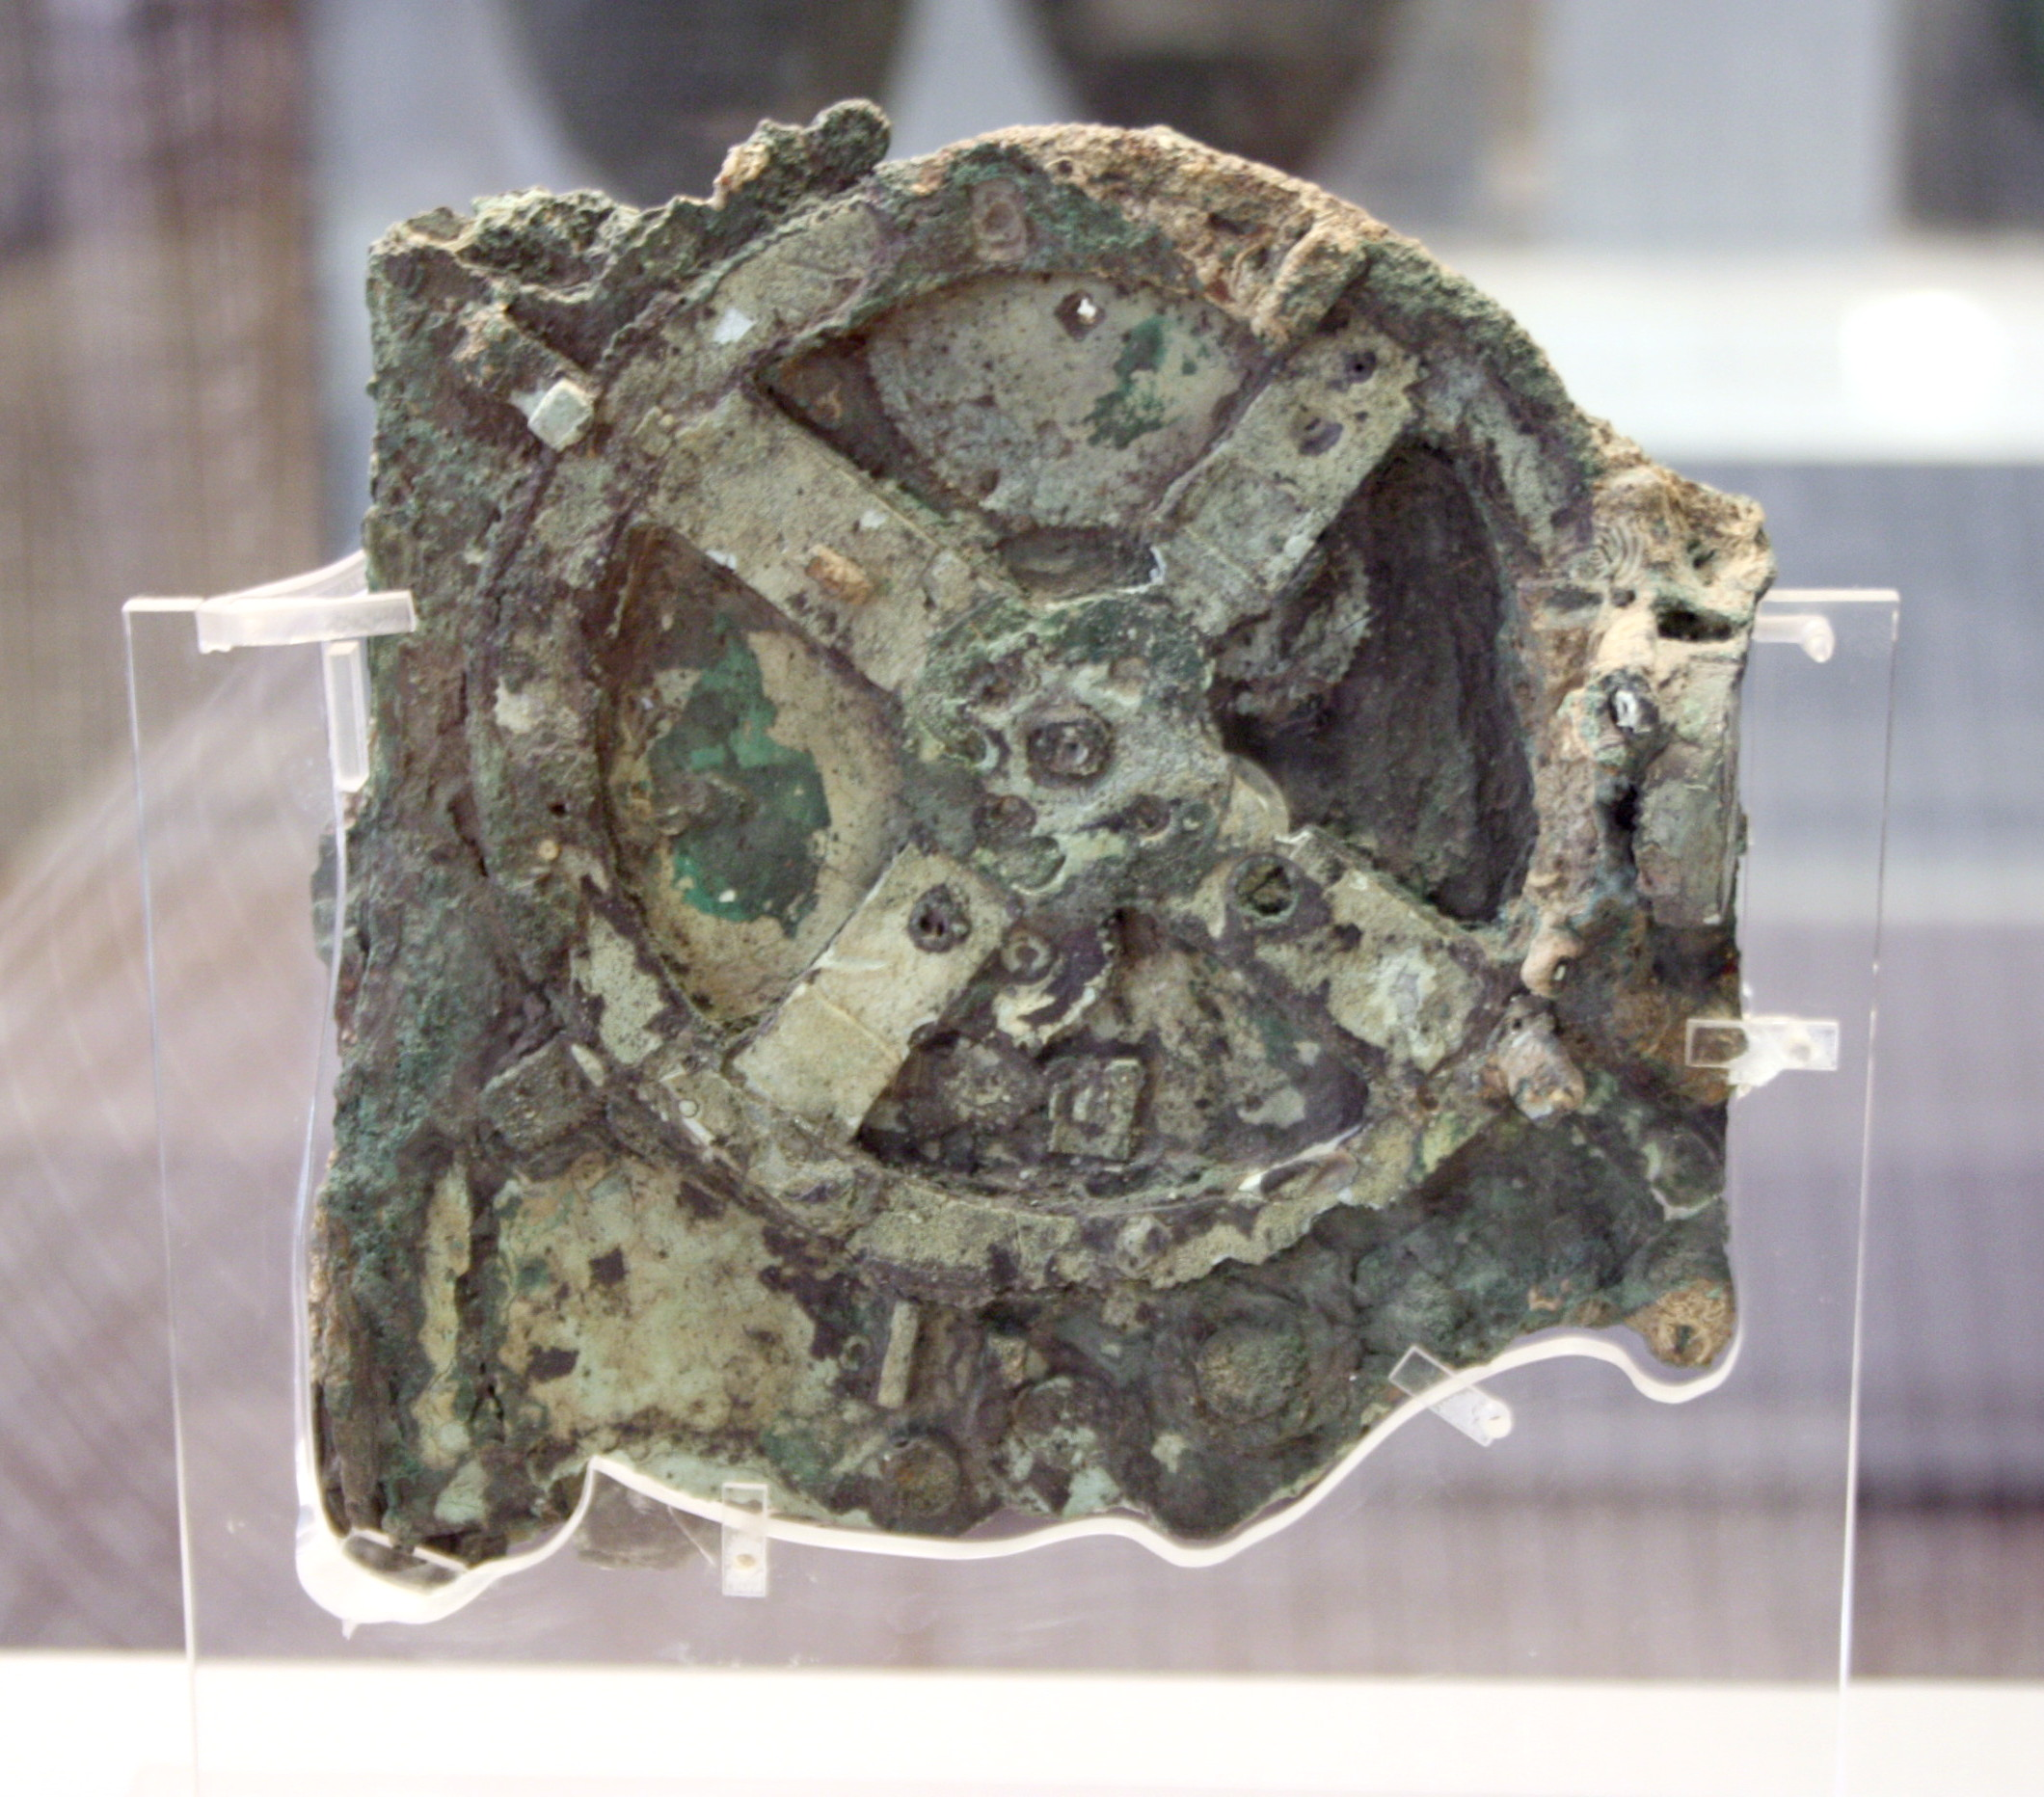
\includegraphics[width=5in]{antikythera_photo.jpg}
\caption{The Antikythera Mechanism at the National Archaeological Museum, Athens---Giovanni Dall'Orto}
\label{atikytheraphoto1}
\end{figure}

\begin{figure}
\centering
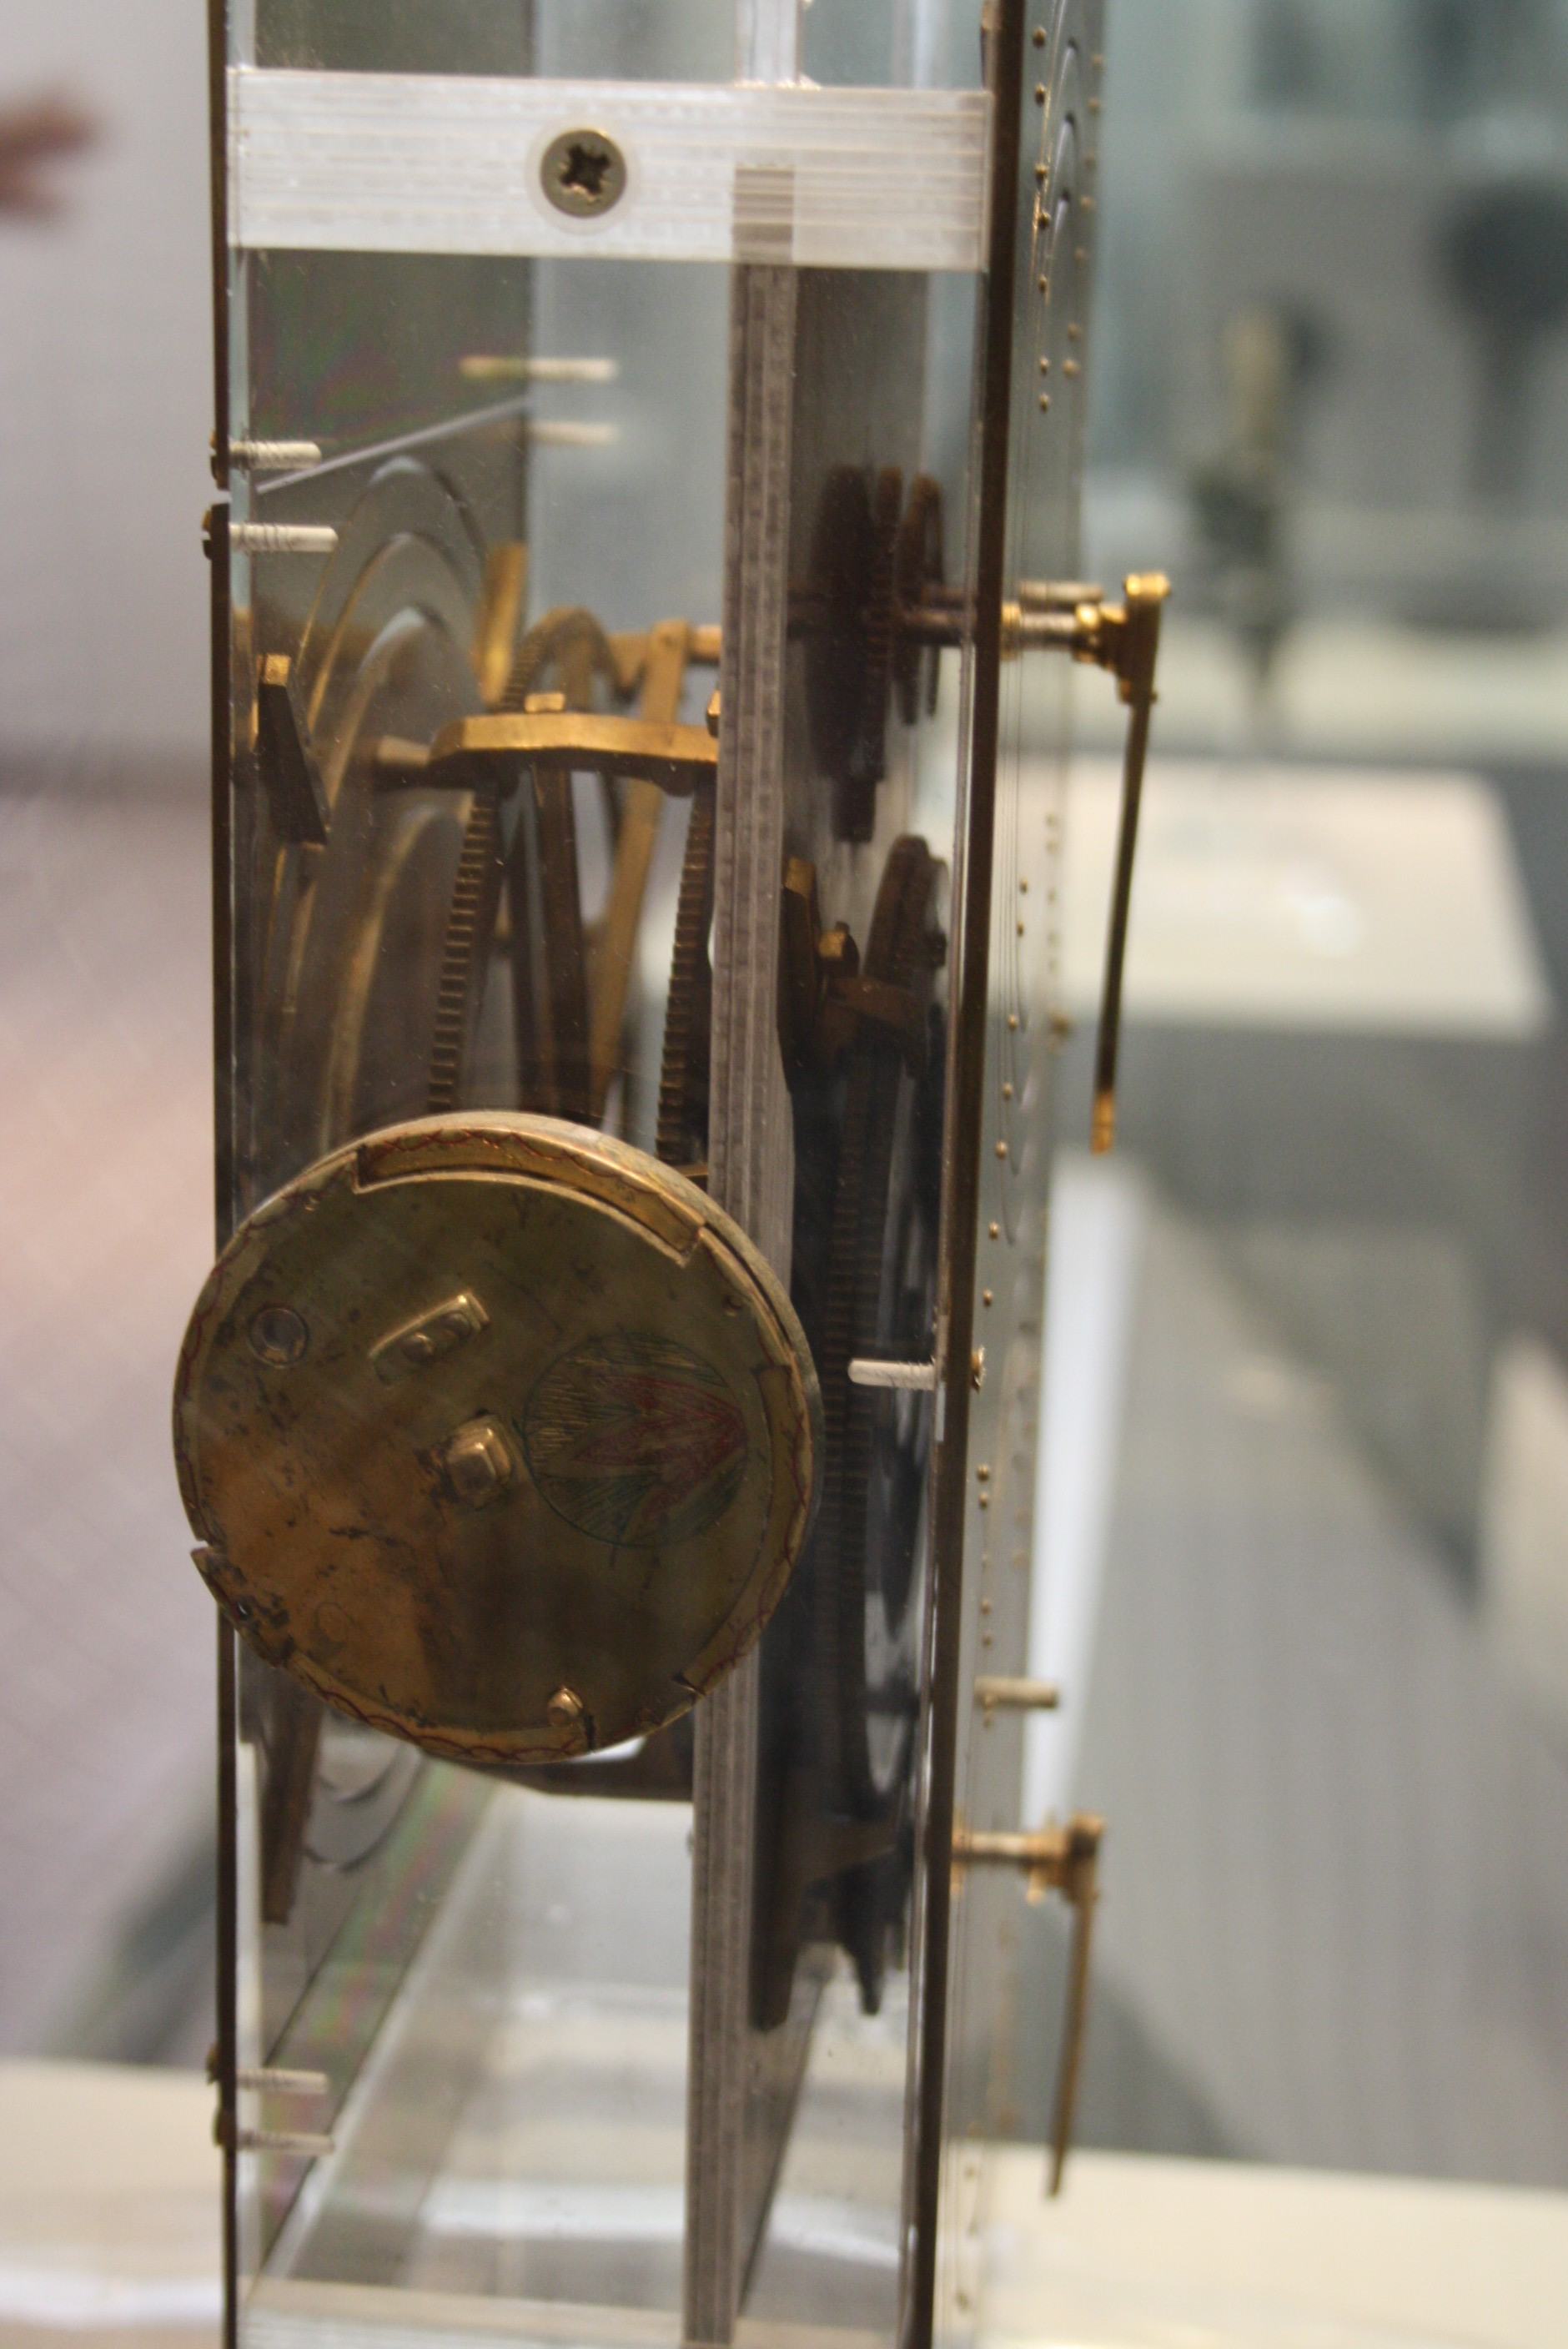
\includegraphics[width=5in]{antikythera_reconstruction_photo.jpg}
\caption{Reconstruction of the Antikythera Mechanism at the National Archaeological Museum, Athens---Giovanni Dall'Orto}
\label{antikytherareconstruction1}
\end{figure}

\index{reverse engineering!techniques!contextual}
Jo Marchant details the entire story of the reverse engineering of the
Antikythera device in a fascinating book \citep{marchant2009}. A
significant amount of design recovery was accomplished in terms of the
purpose of the device and the identity and thinking of the original
engineer(s). Referring to Greek letters engraved on the casing of the
device, she writes, “[The reverse engineer] also noted that the letters
were so precise they must have been engraved not by a labourer but by a
highly trained craftsman” \citep[][p.~55]{marchant2009}. She also recognized that
the incorporation of historical and cultural information from the time
period was valuable for unlocking some of the mysteries of the device.
As an example, consider the following passage, “archeologists also
studied the rest of the salvaged cargo. Their discoveries help to paint
a vivid picture of when the ship sailed, where her load was being
taken, and the sort of world from which she came. From there we can
guess at the origins of the Antikythera mechanism itself, and how it
ended up on its final journey” \citep[][p.~61]{marchant2009}. Thus, it is clear
that reverse engineering is most effective when all pertinent
information is brought to bear. This is accomplished by looking at the
“big picture” instead of limiting the study to the narrow set of data
obtained by simply dissecting the specimen.\footnote{
For more details on this idea, see Dominic Halsmer
and Jessica Fitzgerald, ``Metaphysical Considerations Enhance Reverse
Engineering Studies,'' presented at the ASA Annual Meeting, North
Central College, July 29-August 1, 2011 \citep{halsmerfitzgerald2011}, and for a discussion of the
incorporation of the concept of corruption, see Dominic Halsmer and
Sean McDonough, ``Affordance-based Reverse Engineering of Natural
Systems with Possible Corruption,'' Proceedings of the 2011 Christian
Engineering Education Conference (CEEC), Trinity Western University,
June 29-July 1 \citep{halsmermcdonough2011}.
}
\index{Antikythera device|)}

Dennett’s approach to reverse engineering through optimality
considerations has recently been criticized from a couple directions.
Philosopher Robert Richardson contends that such an approach to
evolutionary psychology lacks the standard level of evidential support
enjoyed by evolutionary biology. Refer to his recent
book \citep{richardson2007} for details of his criticisms. A second
criticism, that gets more to the heart of the matter, looks
specifically at Dennett’s insistence on optimality as the guiding
beacon of the reverse engineering enterprise. Philosophers Krist Vaesen
and Melissa van Amerongen have recently published an extensive analysis
of Dennett’s artifact hermeneutics. They argue that “Dennett’s account
is implausible{\ldots} [and] conclude that, quite in contrast to Dennett,
intentional considerations play a crucial role in artifact
hermeneutics, and even stronger, are necessary for the sake of
simplicity and precision” \citep[][p.~779]{vaesenamerongen2008}.

\index{reverse engineering!intent}
Vaesen and van Amerongen claim that artifacts should be interpreted by
relying both on optimality and intentional considerations, recognizing
that this hampers Dennett’s strategy of reverse engineering artifacts
and organisms in the same way \citep[][pgs. 794--795]{vaesenamerongen2008}. Their thoughts on
how Dennett’s unified approach might still be achieved leads to an
interesting final paragraph. They write,

\begin{quote}
Of course, it still might be
possible to establish a generic interpretive program, including
artifacts \textit{and} biological items… What is needed to argue for
the importance of intent in the interpretation of organ(ism)s, is a
proof that intent reveals things that remain hidden under an optimality
account or that it is beneficial to ignore optimality and dig for a
designer’s – i.e., nature’s – intentions instead. It is far from
evident that such things can be done without entering the waters of
creationism. Fortunately, the burden of proof is on, if any, those who
think our understanding of biofunctions is – or should be – linked to
“Mother Nature’s” intentionality.  \citep[][p.~795]{vaesenamerongen2008}
\end{quote}

Vaesen and van
Amerongen’s demand for a \textit{proof} that intent reveals things that
remain hidden under an optimality account is quite a stringent
requirement. In the remainder of this article it should become clear
that, although short of a proof, there is a significant amount of
evidence that this is the case. Considerations of intention while
conducting affordance-based reverse engineering of natural systems do
reveal valuable things that remain hidden and unrealized under
Dennett’s approach.
\index{reverse engineering!techniques!optimality|)}

\section[Design Recovery Techniques]{Reverse Engineering and Design Recovery Techniques}

\index{reverse engineering!epistemology}
If reverse engineering really is a profitable method for studying
natural systems, then this approach should be fully explored to ensure
that maximum benefit is achieved. A valuable resource that discusses
function-based methods for hardware systems is \textit{Product Design:
Techniques in Reverse Engineering} \citep{ottowood2001}.\footnote{
This book details function-based
techniques for reverse engineering of man-made hardware. See Denis L.
Feucht, ``Design in Nature and the Nature of Design,''\citep{feucht1999} 
for a discussion of the relevance of
functional theories to the design of living organisms.
} However, a more
concise, yet detailed description of the process is found in an article
entitled ``On Reverse Engineering'' by M. G. Rekoff,
Jr \citep{rekoff1985}. He describes a method for systematically
conducting the reverse engineering activity, noting that it ``is not
really greatly different from that of detective work in a criminal
investigation or of conducting military intelligence
operations.''\citep[][p.~245]{rekoff1985} In a nutshell, Rekoff recommends the
decomposition of existing structural hierarchy in developing functional
specifications until the mechanism-of-operation is completely
understood. This is unpacked in the following steps of his grand plan
for conducting a reverse engineering effort{\ldots}

\begin{itemize}
\item 
``System-engineer'' [analyze the interconnectivity with an engineering
mindset] first to establish hypotheses based on the information
presently at hand and to identify the measurement/test needs.
\item 
Disassemble to the extent required to verify or modify the hypotheses
and to perform supporting tests. One will not only uncover information
relating to the hypotheses but will possibly also uncover information
that was not previously known to exist.
\item 
Further ``system-engineer'' on the basis of all the information in hand,
form new hypotheses, and prepare for additional measurement and
testing.
\item 
Further disassemble, measure, and test to validate hypotheses and
uncover new information.
\end{itemize}

This process continues until the degree of understanding is adequate for
the purposes of the reverse engineering effort. For any particular item
within the overall system being analyzed, “the generic process consists
of the following five sequenced steps; assimilate existing data;
identify elements; disassemble; analyze, test, and dimension; and
complete documentation.” Each of these steps is explained in very
helpful detail in Rekoff’s previously-referenced article.

\index{reverse engineering!design recovery}
Another helpful article, although dealing mainly with the reverse
engineering of computer software, introduces the concept of ``design
recovery.'' ``Reverse Engineering and Design Recovery: A Taxonomy'' by
Elliot Chikofsky and James Cross defines design recovery as ``a subset
of reverse engineering in which domain knowledge, external information,
and deduction or fuzzy reasoning are added to the observations of the
subject system to identify meaningful higher level abstractions beyond
those obtained directly by examining the system
itself.''\citep{chikofskycross1990}
In other words, the goal of design
recovery is to work out, at a higher level of understanding, what a
system or component was engineered to do, and (to some degree of
confidence) why, rather than just examining its subcomponents and their
interrelationships. This generally involves extracting design
artifacts, by detecting design patterns for example, and synthesizing
abstractions that are less dependent on implementation. The authors
believe that it is these higher level abstractions that are the key to
fully reverse engineering complex natural systems. In another article,
Ted Biggerstaff further expounds on the idea, ``Design recovery
recreates design abstractions from a combination of code [system],
existing design documentation (if available), personal experience, and
general knowledge about problem and application domains{\ldots}Design recovery
must reproduce all of the information required for a person to fully
understand what a program [system] does, how it does it, why it does
it, and so forth.''\citep{biggerstaff1989}

\index{reverse engineering!design recovery}
\index{reverse engineering!techniques!top-down}
\index{reverse engineering!techniques!bottom-up}
\index{design!abstract design concepts}
\index{reverse engineering!abstract design}
A design recovery framework for mechanical components that was recently
developed by engineering researchers at the University of Windsor in
Canada appears to be a promising and comprehensive approach to this
problem that may be transferrable to natural systems. R. Jill Urbanic
and Waguih ElMaraghy contend that 

\begin{quote}
there must be a methodology for
recognizing design intent. The feature shapes are not arbitrary, nor is
their pattern of arrangement{\ldots}A form-function link needs to be
established at different levels of granularity to infer the designer’s
intent{\ldots}The proposed framework includes mapping from the application
domain to the functional requirements and integrates the bottom-up
reverse engineering and top-down forward engineering processes and
perspectives. The objective is to be able to develop a fully described
model that considers the abstract design concepts and rationale along
with the specific physical details. \citep{urbanicelmaraghy2009}
\end{quote}

\index{reengineering}
\index{value engineering}
\index{reverse engineering!design recovery}
\index{reverse engineering!biology}
\index{human condition}
\index{worldview}
\index{salvation}
\index{redemption}
\index{apologetics}
\index{Christian witness}
The framework developed in this paper is utilized to conduct
reengineering (or value engineering – improving a system based on a
reverse engineering analysis) in a subsequent paper by this group. Here
they claim that “gathering this [design recovery] information allows
the [reverse engineer] the means to make informed decisions as to
whether the current component design is adequate, or how may it be
modified to add value” \citep[][p.~166]{urbanicelmaraghy2009b}. In her 
book \textit{Reverse Engineering}, Kathryn Ingle emphasizes the importance of design
recovery data for reengineering. She writes, “This is no small amount
of information if a future attempt at value engineering is to be made.
Knowledge of the hows and whys of a part’s design allows the [reverse]
engineer to make quantum leaps in thought when seriously contemplating
value engineering” \citep[][pgs. 65--66]{ingle1994}. As researchers increasingly
apply reverse engineering to living systems,\footnote{
As examples see Simon Polstra et al., “Towards
Design Space Exploration for Biological Systems” \citep{polstraetal2008}
and Jamal O. Wilson and David Rosen,
“Systematic Reverse Engineering of Biological Systems” \citep{wilsonrosen2007}.
} a
natural extension will involve the application of value engineering to
human beings and the fundamental problem of the human condition. As
\textit{Christian} engineers/scientists, who are aware of the ultimate
solution to this problem, we should be ready to present this solution
in a way which people can understand, especially other
engineers/scientists.\footnote{
For more thoughts along these lines, see Harold
Heie, “Christian Engineers as Faithful Witnesses to God’s Redemptive
Purposes for Creation” \citep{heie1999}
and Walter L. Bradley,
“Is There Scientific Evidence for an Intelligent Creator of the
Universe?” \citep{bradley2003}
and Dominic M. Halsmer, “Why Engineers Make Good Apologists” \citep{halsmer2007},
 and Dominic M. Halsmer, Jon Marc Asper, and Ben Zigrang,
“Enhancing Science and Engineering Programs to Equip and Inspire
Missionaries to Technical Communities” \citep{halsmeretal2011},
and Dominic M. Halsmer,
“Application of the ‘Engineering Mindset’ for Worldview Evaluation” \citep{halsmer2009},
and Stephen T. Frezza, “Deus Machinator: God the Engineer” \citep{frezza2009}.
} One approach is to
demonstrate the rational (though not absolutely compelling) basis for
such a life-changing decision by couching it in terms of the mature
fields of reverse engineering and value engineering. This strategy is
enhanced further by incorporating the concept of affordance into the
reverse engineering process. These ideas will be explored further in
the later part of this paper.

\section{Affordance-based Reverse Engineering}

\index{design theory}
\index{affordances|(}
\index{design theory!affordances|(}
\index{form}
In a recent article in \textit{Mechanical Engineering}, Jonathan Maier
calls for a rethinking of design theory by emphasizing that design
problems begin at the system level. He claims that ``individual
components can be designed only after the whole problem has been
understood and defined at the system level and then decomposed into
subsystems and so forth, down to individual components that can be
designed using the hard engineering sciences and traditional analysis
methods'' \citep[p.~34]{maier2008}\citep{maier2011}. Major engineering projects have become so
complex and far-reaching that George Hazelrigg has argued that design
is no longer just multidisciplinary; it is \textit{omni-disciplinary}
in that any and all disciplines may be involved in the solution to a
particular design problem \citep{hazelrigg1996}. Maier is convinced that
the complexities of systems thinking and user interactions require
design engineers to move beyond the level of simply designing for
component or product function. The concept that he proposes is
\textit{affordance}, which is what a system provides to a user or to
another system. An (positive) affordance is what something is “good
for” or “good at”, and may serve as an underlying and unifying
principle in the science of design \citep{maierfadel2001}. It is important
to note that the affordances of a system depend on the physical form of
the system, whereas the functions of a system do not. This is a useful
feature “because it allows engineers to analyze and compare the
affordances of product concepts (especially at the system level) as
well as of existing products for reverse
engineering” \citep[][p.~36]{maier2008}.

\index{psychology!gestalt}
\index{gestalt|see{psychology, gestalt}}
\index{reverse engineering!roles}
Although the term “affordance” has its roots in Gestalt
psychology\citep{koffka1935}, perceptual psychologist James Gibson
defined it in the modern era as “what it [the environment]
\textit{offers} the animal [user], what it \textit{provides} or
\textit{furnishes}, either for good or ill{\ldots}I mean by it something that
refers to both the environment and the animal [user] in a way that no
existing term does. It implies the complementarity of the animal [user]
and the environment” \citep[][p.~127]{gibson1979}. Donald Norman, in his book
\textit{The Design of Everyday Things}\citep{norman1988}, steers the
concept toward engineering design, but stops short of Maier’s
contention that it is fundamental to the design or reverse engineering
of any artifact. However, Norman does admit that “affordances provide
strong clues to the operations of things.” Maier emphasizes that the
affordance-based approach to design captures important interactions
within the engineer-artifact-user triad that the function-based
approach misses. In reverse engineering applications, a fourth role
must be added to the triad---that of the investigator, or reverse
engineer. Interesting interactions may be elucidated among these four
roles by incorporating the concept of affordances. Maier compares the
strengths and weaknesses of function-based and affordance-based design
and comes to an interesting conclusion; there are several “appealing
synergies” or “ways in which strengths of function complement
weaknesses of affordance, and ways in which the strengths of affordance
complement the weaknesses of function” \citep{maierfadel2002}. These
synergies include a better view of “the big picture,” a uniting of
design methods, and a theoretical underpinning of design that
illuminates the proper role of function.

\index{affordances!artifact-user-affordances}
\index{affordances!artifact-artifact-affordances}
\index{affordances!negative affordances}
\index{affordances!affordance structure matrix}
In further work by Jonathan Maier and Georges Fadel on affordance-based
methods for design and reverse engineering, they describe two kinds of
affordances. Artifact-user-affordances (AUA) are defined as “the set of
interactions between artifact and user in which properties of the
artifact are or may be perceived by the user as potential uses. The
artifact is then said to \textit{afford} those uses to the user. Now we
can define artifact-artifact-affordances (AAA) as the set of
interactions between two artifacts in which some properties of one
artifact interact in some useful way with properties of the other
artifact” \citep{maierfadel2003}. In addition, they explain how both types
of individual affordances can be considered as positive or negative
depending on whether the interaction is good for the system or not.
Furthermore, each affordance can have a quality of interaction
associated with it depending on how well the interaction serves its
role. For example, a chair may afford sitting much better than a large
rock, and the weight of a large rock may be seen as a negative
affordance if portability is an issue. Maier and Fadel claim that a
systematic evaluation of the affordances of each part of a system can
be combined into a comprehensive affordance structure matrix (ASM),
including both AUA and AAA \citep{maieretal2003, maieretal2008}. The system is then
effectively reverse engineered in the sense that its operation is well
understood. The ASM lists system components on a horizontal axis and
affordances along a vertical axis. The matrix is populated by
identifying which components are associated with each affordance.
\index{affordances|)}
\index{design theory!affordances|)}

\section[How Affordances Assist]{How Affordances Assist in the Reverse Engineering of Natural Systems}

\index{control theory}
\index{modularity}
\index{systems biology|(}
\index{protocols}
\index{affordances!artifact-artifact-affordances}
In March of 2002, the cover story for \textit{Science} was entitled
``Reverse Engineering of Biological Complexity,''\citep{csetedoyle2002}
which encouraged the application of engineering concepts like those
borrowed from control theory to better understand the complex workings
of biological systems. The article also emphasized the modularity and
protocols that were being discovered within such systems at the time.
Protocols were described as ``rules that prescribe allowed interfaces
between modules, permitting system functions that could not be achieved
by isolated modules.'' Thus, understanding interacting modules and the
protocols that specify those interactions is critical to identifying
the affordances between modules (AAA). An interesting analogy was drawn
between biological structures and the modules and protocols of the Lego
toy system, demonstrating in multiple ways how biological systems
exhibit features that are readily associated with engineered devices.
The article concludes by encouraging biologists and engineers to
``compare notes.'' Since this paper was published, it seems that many
have been doing just that. 

\index{reverse engineering!biology}
\index{affordances!identification}
\index{E. coli}
\index{heat shock response}
\index{protocols}
\index{biology!protocols}
\index{biology!information pathways}
\index{reverse engineering!information pathways}
\index{affordances!comprehensibility}
Physiologist Robert Eisenberg comments that it is most helpful to “look
at biological systems through an engineer’s eyes” \citep[][p.~376]{eisenberg2007}.
Emphasizing how this leads to successful experimentation, he writes,
“But it seems clear, at least to a physiologist, that productive
research is catalyzed by assuming that most biological systems are
devices. Thinking today of your biological preparation as a device
tells you what experiments to do tomorrow.” Many of these types of
experiments serve to identify affordances. At Stanford University, an
aerospace engineer, Claire Tomlin, and a molecular biologist, Jeffrey
Axelrod, teamed up to extol recent efforts aimed at
``understanding biology by reverse engineering the
control'' \citep[][pgs. 4219--4220]{tomlinaxelrod2005}. They summarize an extensive reverse
engineering study of the mechanism used by bacterium E. coli to combat
heat shock \citep{elsamadetal2005}, claiming that it “is just what a
well-trained control engineer would design, given the signals and the
functions available.” Viewing the heat shock response as a control
engineer would, the researchers developed a reduced order mathematical
model to analyze the dynamics of each of the interacting modules. This
analysis then motivated a series of simulation experiments on a larger
mathematical model. The experiments involved disconnecting one or more
information pathways (both feedback and feedforward protocols) which
allowed comparison of various closed-loop and open-loop responses. As a
result, they obtained a clearer picture of how certain information
pathways and protocols afforded robustness, efficiency, and noise
attenuation. Tomlin and Axelrod claim that this analysis 

\begin{quote}
is important
not just because it captures the behavior of the system, but because it
decomposes the mechanism into intuitively comprehensible parts. If the
heat shock mechanism can be described and understood in terms of
engineering control principles, it will surely be informative to apply
these principles to a broad array of cellular regulatory mechanisms and
thereby reveal the control architecture under which they
operate{\ldots}Certainly these kinds of analyses promise to raise the bar for
understanding biological processes.
\end{quote}

\index{systems biology|)}

\section{Affordances for Human Life}

\index{affordances!human|(}
\index{worldview}
\index{imago dei}
\index{cosmology}
\index{God, as engineer}
In order to illustrate the application of this approach to even more
complex natural systems, consider the further example of a human being.
Is it possible, or even reasonable, to apply reverse engineering and
design recovery techniques in an effort to gain insight into this
system?\footnote{
A very interesting and extensive attempt at reverse
engineering human life is documented in Bryant M. Shiller,
\textit{Origin of Life: The Fifth Option},\citep{shiller2004}
which finishes with the surprising conclusion that an alien
intelligence is using humanity as a self-perpetuating and robust
information storage system.
} Of course, this approach assumes the
possibility of a designer whose products lend themselves to such
techniques. Multiple popular worldviews adhere to the existence of a
master engineer/architect of some kind, and the point was made earlier
that complex natural systems are currently being successfully reverse
engineered. Thus, this seems like an interesting and fruitful pursuit.
This approach is especially fitting under the further assumption that
humans are “made in the image” of such a master engineer, which is
characteristic of a Christian worldview. This would presumably help to
explain why there is such a profitable match between the complexity of
the cosmos and the mental capabilities of humans. Such a
match forms the basis for any successful reverse engineering of natural
systems. However, the Christian worldview also entails the existence of
an adversary who opposes the work of the master engineer, which may
make the reverse engineering task more challenging.

\index{reverse engineering!roles}
The first step is to define the roles of artifact, user, investigator,
and engineer that make up the big picture of design and reverse
engineering. For this case the artifact can be considered as the human
being, although it is difficult to separate humans from their finely
tuned cosmic environment. The end user is the human mind, or
consciousness, in the sense that human minds make use of use their
bodies in living their lives. In a Christian worldview, there is also a
sense in which God is the end user, since he has made all things for
himself. The investigator, or reverse engineer, is anyone who is
curious enough to pursue this kind of study. It is important to
recognize this so that the investigator can limit his or her
bias that affects their analysis. Admittedly, there is some overlap among
these roles, but that should not negate the potential fruitfulness of
this analysis. As for the engineer, whether it is the tinkerer of
naturalism, or God, or space aliens, it is hoped that more can be
discovered about this engineer’s motives, methods and intentions (or
lack thereof) by properly applying the reverse engineering process. 

\index{affordances!cosmological}
Just listing all the affordances that the universe (artifact) exhibits
towards the human consciousness (user) would be a complex and
time-consuming task, but by looking at those that are the most
significant, insights can begin to be gleaned. To start off, the cosmos
affords humans with the ability to learn. By studying the universe and
its interactions, such as those between stellar bodies, molecules, or
light, humans are able to gain knowledge about why previous natural
events occurred the way they did, and predict how future events might
follow the same pattern. The human mind is able to experience these
because of the sensory organs, which the human body affords to the
human mind.

\index{affordances!human body}
This brings up an interesting question; what else does the human body
afford the consciousness? According to Oxford Philosopher Richard
Swinburne \citep[][p.~169]{swinburne2004}, in order to be able to interact and
learn about the environment in which it is placed, and yet still be a
humanly free intelligence, the mind needs the human body to contain:

\begin{enumerate}
\item Sense organs with enormous capacity to receive information regarding
distant world states.
\item An information processor to turn sense organ states into brain states
(resulting in beliefs).
\item A memory bank to file states correlated with past experiences (needed
to reason).
\item Brain states that give rise to desires, both good and evil.
\item Brain states caused by many different purposes that we have.
\item A processor to turn these states into limb and other movements
(needed to act on purposes).
\item Brain states that are not fully determined by other physical states
(needed for free choice).
\end{enumerate}

\index{affordances!cosmological}
\index{cosmology!initial conditions}
\index{cosmology!fine tuning}
Another affordance that the universe provides the human consciousness is
an environment to thrive in.\footnote{
In James V. Schall, \textit{The Order of Things}, 83, the author writes, ‘To be
allowed “a place on earth” wherein to work out the distinction of good
and evil is what, in the end, the cosmos and earth seem to be about’ \citep[][p.~83]{schall2007}.
} One key aspect of the
universe is the fact that it is so finely tuned.\footnote{
In Alister E. McGrath, \textit{A Fine-Tuned
Universe: The Quest for God in Science and Theology}, the author makes the point that not
only is the universe fine-tuned for life, but human beings are
fine-tuned to profitably interact with the universe. Regardless of how
this came about, the result has significant philosophical and
theological implications \citep{mcgrath2009}.
} As
Swinburne states, 

\begin{quote}
Not all initial conditions (ICs) or laws of nature
would lead to, or even permit, the existence of human bodies at some
place or other, and at some time or other, in the universe. So we may
say that the universe is `tuned' for the evolution of human bodies if
the laws and initial conditions allow this to occur. If only a very
narrow range of laws and ICs allow such evolution, then we may say that
the universe is `fine-tuned' for this evolution. Recent scientific work
has shown that the universe is fine-tuned. \citep{swinburn2004}
\end{quote}

Now, the existence of the human body, due to these fine tuned conditions
is an important aspect of human consciousness because of the
affordances mentioned above. What is even more amazing is that the fine
tuning of the universe not only allows for life, but allows for persons
who are able to question why the universe is the way it is. The
fine-tuning of the universe then also affords the human consciousness
with the ability to discover attributes of the engineer by questioning
and observing how something so encompassing as the cosmos can be so
elegant and well-engineered. With this in mind, the investigator can
then appreciate the overlap with the area of the user as the human
consciousness.

\index{reverse engineering!roles}
\index{biology!flagellum|see{bacterial flagellum}}
\index{bacterial flagellum}
\index{flagellum|see{bacterial flagellum}}
\index{affordances!biology}
Considering that the user and investigator are roles filled by the same
person brings a new dynamic and even more complex affordances between
the different components of the system. As the investigator, the human
consciousness begins to question why things are the way they are within
the system, and if there is any way to improve the system. Humans have
been attempting this from the beginning of conscious thought with
innovations and inventions meant to increase the quality of life.
Recently, what scientists have discovered is that many of these new
inventions have already existed in nature. A prime example of this is
the boat propeller and the bacterial flagellum. 

\index{affordances!perception of}
\index{semiotics|see{biology, semiotics}}
\index{biology!semiotics}
\index{nature!meaning in}
\index{transitive complexity}
The ability of humans to not only perceive affordances but also imagine
how they might be creatively achieved is discussed in an article
entitled ``Affordances are Signs''\footnote{
McGrath also picks up on this
theme in \textit{A Fine-Tuned Universe: The Quest
for God in Science and Theology}, writing, ``The emergence of the discipline of semiotics
has encouraged us to see natural objects and entities as signs,
pointing beyond themselves, representing and communicating themselves.
To find the true significance of things requires the development of
habits of reading and directions of gaze that enable the reflective
observer of nature to discern meaning where others see happenstance and
accident. Or to use an image from Polanyi, where some hear a noise,
others hear a tune” \citep[][p.~3]{mcgrath2009}. In David Seargent, \textit{Planet Earth and the
Design Hypothesis}, the author defines a
type of complexity found in nature as “transitive complexity” if it
serves as a sign that points to a “larger state of affairs beyond
itself” \citep{seargent2007}.
} by psychologist
John Pickering \citep{pickering2007}. He asserts, 

\begin{quote}
The characteristic reflexivity of the
human condition means that we are not only able to perceive the world
as it is, that is, to perceive the affordances that actually surround
us, but also to perceive affordances that do not yet exist, that is, to
perceive the world as if it were otherwise. When we take a rock and
modify it with blows until it functions as a blade, we do just that. We
not only perceive what is, but also what may be and hence we may take
meaningful, intentional action to bring it about if we so choose. \citep{pickering2007}
\end{quote}

\index{recursion}
\index{self-organization}
\index{autopoiesis}
\index{self-improvement}
\index{epistemology}
\index{systems theory}
\index{systems theory!epistemology}
\index{kingdom of God}
The
interesting thing that Swinburne points out is that the choices humans
make not only tend to affect the world and others around them, but also
affect their own characters (recursion), giving them some measure of
influence over the kinds of people they eventually become. This is a
very interesting affordance, which when coupled with the human ability
to envision a preferable future, leads people to form various purposes
related to self-organization (autopoiesis) and self-improvement.
However, a common experience among humans is the inability to realize
accepted standards and expectations. In an article entitled “The
Kingdom of God and the Epistemology of Systems Theory: The Spirituality
of Cybernetics” \citep{buker2009}, William Buker, a Professor of
Counseling, suggests that features of the human condition such as
recursion and autopoiesis, combined with the nature of the universe,
serve to invite humans into a more complementary coupling with the
larger mind of the master engineer. He also points out how this idea of
fitting with the environment rather than fighting against it is
consistent with Jesus’ message of the kingdom of God.

\index{epistemology}
\index{humanity!purpose}
\index{spirituality}
\index{love}
\index{transcendentals}
\index{humanity!community}
Obviously, such possibilities require the recognition of valid
epistemologies beyond those of science and history, such as are found
in human experiences of joy, faith, hope, and love. Some researchers
are suggesting that it is time to more fully explore the wide breadth of
knowledge found in the human condition if a clearer picture of
mankind’s purpose and place in the universe is to be achieved.
Alexander Astin, Founding Director of the Higher Education Research
Institute at UCLA, argues that spirituality deserves a central place in
higher education \citep{astin2004}. He claims that ``more than
anything else{\ldots}[this] will serve to strengthen our sense of
connectedness with each other{\ldots}This enrichment of our sense of community
will not only go a long way toward overcoming the sense of
fragmentation and alienation that so many of us now feel, but will also
help our students to lead more meaningful lives as engaged citizens,
loving partners and parents, and caring neighbors.'' At the beginning
point of this reverse engineering project, perhaps it is too early to
speculate about indications of the ultimate purpose for mankind, but it
seems that Dr. Astin has put his finger on the pulse of what may be
humanity’s greatest desire, function and purpose; that of love. A
scientific perspective of love is currently being pursued by the
Institute for Research on Unlimited Love at Case-Western Reserve
University. Thomas Jay Oord, theologian for the institute, has written
extensively on this topic, including \textit{Science of Love: The
Wisdom of Well-Being} \citep{oord2004}. He says that
“to love is to act intentionally, in
sympathetic response to others (including God), to promote overall
well-being.” Given the high value that humanity has placed on love
throughout history, and its power to change lives for the better, it is
hard to imagine that, if humans do have purpose, it would not have
something to do with love. One example of a scientifically rigorous and
testable model of the cosmos, which postulates the love of a master
engineer and encourages humans to return that love as part of their
primary purpose, is documented in the book
\textit{More than a Theory},\citep{ross2009}
by astronomer Hugh Ross.
\index{affordances!human|)}

\section{Implications for Worldview}

\index{worldview|(}
\index{affordances!cosmological}
\index{cosmology}
\index{cosmology!interconnections}
\index{design recovery!cosmology}
\index{reverse engineering!roles}
The advance of science in several areas is helping to identify the many
affordances that the cosmos provides for higher life forms like human
beings \citep{barrow2008}. These affordances are facilitated by the
integration of the many subsystems of our world, which also exhibits
affordances between subsystems. The connectedness of the universe is
aptly described in the following quote by the famous naturalist, John
Muir, “When we try to pick out anything by itself, we find it hitched
to everything else” \citep[][p.~110]{muir1988}. Some scientists have suggested
that such affordances can lead us to a clearer understanding of
worldview, and human meaning and purpose \citep{denton1998}. This is
not surprising since that is ultimately what reverse engineering and
design recovery procedures were designed to detect; what was the
original engineer thinking? It is clear that the application of reverse
engineering to natural systems cannot be separated from the worldview
of the investigator because the concept of an engineer is critical to
the study. Recall the importance of the relationships between engineer,
artifact and user in this regard. The authors have suggested that there
is another entity that should be included in this grouping; the
investigator, or reverse engineer. In fact, the worldview of the
reverse engineer, while playing a role in the study, may also be
further shaped in the midst of the study. A classic example is the case
of Charles Darwin, who, early in his career, greatly admired the works
of natural theology, such as penned by William Paley, while later on,
he expressed doubts as described in his writings.\footnote{
\index{Darwin, Charles}
In C. R. Darwin, \textit{The Life and Letters of
Charles Darwin}, edited by his son, Charles Darwin writes, 

\begin{quote}
I cannot see as plainly as others do,
and as I should wish to do, evidence of design and beneficence on all
sides of us. There seems to me too much misery in the world.  I cannot
persuade myself that a beneficent and omnipotent God would have
designedly created the Ichneumonidae with the express intention of
feeding within the living bodies of caterpillars, or that a cat should
play with mice…On the other hand, I cannot anyhow be contented to view
this wonderful universe, and especially the nature of man, and to
conclude that everything is the result of brute force. I am inclined to
look at everything as resulting from designed laws, with the details,
whether good or bad, left to the working out of what we may call
chance. Not that this notion at all satisfies me. I feel most deeply
that the whole subject is too profound for the human intellect. A dog
might as well speculate on the mind of [Isaac] Newton. Let each man
hope and believe what he can. \citep{darwinll}
\end{quote}
}

\index{reverse engineering!worldview implications}
\index{worldviews!testability}
\index{humanity!purpose}
In teaching the process of reverse engineering, and applying it to
natural systems, it must be recognized that worldview plays an
important role, and that worldview implications may result. The
particular worldview of an investigator may, or may not, facilitate
discovery and reverse engineering in natural systems. The extent to
which a worldview is helpful in this regard is simply the extent to
which a worldview is an accurate understanding of reality. Care should
be taken to allow students and investigators to shape their worldviews
in accordance with the evidence. Worldviews are determined based on
various kinds of evidence and experiences, but scientific evidence
typically plays a major role. The fact that the natural world is so
readily and profitably reverse engineered suggests that the cosmos
actually is an engineered system; it is the work of a Mind with
extraordinary engineering expertise. Investigators should not hesitate
to consider this perspective, since it not only seems to facilitate
discovery, but may also provide a sublimely satisfying understanding of
personal meaning and purpose.

\index{God!as engineer}
\index{interdisciplinary education}
\index{humanity!purpose}
\index{wordlview!integration}
A research study involving undergraduate honors students and faculty
from a diversity of academic fields, including engineering, theology,
psychology, engineering physics, music, biology, chemistry and
biomedical engineering is currently underway at Oral Roberts
University \citep{halsmerbeck2012}. The students engage in weekly
extra-curricular research and discussions centered on the hypothesis of
“God as Engineer.” This hypothesis is continuously evaluated in light
of a serious engagement with mainstream scientific understandings as
well as a respect for traditional religious truth claims. Students
assess research in the sciences, mathematics, humanities, theology, and
reverse engineering methodologies for applicability to the hypothesis
in question. Weekly meetings are held to discuss findings and develop
journal articles, conference papers and presentations. The diversity of
academic fields represented provides rich and fertile ground for
discussion and conflict resolution. Survey data from current and
previous group participants suggest that these studies help students to
solidify personal integrity, knowledge of purpose, and spiritual
vitality, and enhance their ability to effectively communicate such
convictions.
\index{worldview|)}

\section{Conclusions}

\index{affordances}
\index{reverse engineering!techniques!affordances}
\index{worldview}
\index{cosmology}
\index{purpose}
\index{teleology}
As the concept of reverse engineering is increasingly applied to natural
systems, it will be helpful for students and investigators to
understand the procedures for such studies. Such procedures appear to
be largely absent from the current literature. A reverse engineering
procedure is outlined which makes use of the concept of affordance, a
recent innovation from the field of design engineering. It is suggested
that affordance-based reverse engineering may be particularly useful
when applied to complex natural systems. The example of human life is
briefly discussed. It is recognized that investigator worldview is
inseparable from such reverse engineering studies. Reverse engineering
studies are not conducted in a vacuum. Investigator worldview is
inseparable from such studies. Furthermore, worldview may be
significantly shaped in the midst of such endeavors, since reverse
engineering and design recovery activities ultimately attempt to
identify original meaning and purpose. Anecdotal and survey data from
undergraduate students engaged in such studies generally indicate an
increased appreciation for the affordances of life and the ingenuity
displayed in the cosmos. They also demonstrate an increased ability to
articulate a satisfying and coherent understanding of the meaning and
purpose of human life, as well as the reasons for the hope that they
possess.
\index{reverse engineering|)}

\eandmbibliography{HalsmerLibrary}
